%\renewcommand{\theequation}{\theenumi}
%\begin{enumerate}[label=\thesection.\arabic*.,ref=\thesection.\theenumi]
%\numberwithin{equation}{enumi}
	
\item {\em Proof: }
%\solution
From Fig. \ref{fig:8.1.28},	
%$\triangle AMC \cong \triangle DMB$  by SAS congruency $\because$
%\begin{enumerate}
%\item $AM = BM$
%\item $CM = DM$
%\item $\phase{AMC}$ = $\phase{DMB}$ ( Vertically Opposite Angles)
%\end{enumerate}
%
%\begin{figure}[!ht]
%\centering
%\resizebox{\columnwidth}{!}{

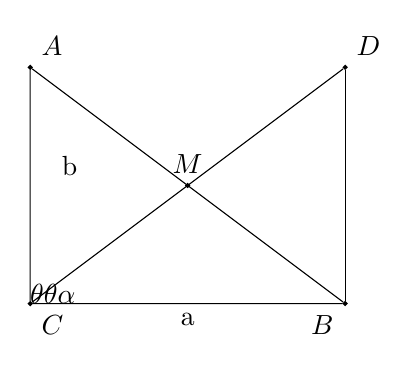
\begin{tikzpicture}
[scale=1,>=stealth,point/.style={draw,circle,fill = black,inner sep=0.5pt},]

%Triangle sides
\def\a{4}
\def\b{3}
\def\c{sqrt(\a^2+\c^2)}



%Labeling points
\node (A) at (0,\b)[point,label=above right:$A$] {};
\node (B) at (\a, 0)[point,label=below left:$B$] {};
\node (C) at (0, 0)[point,label=below right:$C$] {};
\node (M) at (\a*0.5,\b*0.5)[point,label=above:$M$] {};
\node (D) at (\a,\b)[point,label=above right:$D$] {};


%Drawing triangle ABC
\draw (A) -- node[left] {$\textrm{}$} (B) -- node[below] {$\textrm{a}$} (C) -- node[above,xshift=5mm] {$\textrm{b}$} (A);

%Joining CD
\draw (C)--(D);
%Joining BD
\draw (B)--(D);

%Drawing and marking angles
\tkzMarkAngle[fill=orange!40,size=0.5cm,mark=](A,M,C)
\tkzMarkAngle[fill=orange!40,size=0.5cm,mark=](B,M,D)
\tkzMarkAngle[fill=green!40,size=0.5cm,mark=](A,B,C)
\tkzMarkRightAngle[fill=blue!20,size=.2](A,C,B)
\tkzMarkRightAngle[fill=blue!20,size=.2](D,B,C)
\tkzLabelAngle[pos=0.65](A,M,C){$\theta$}
\tkzLabelAngle[pos=0.65](B,M,D){$\theta$}
\tkzLabelAngle[pos=0.65](A,B,C){$\alpha$}


\end{tikzpicture}
}
%\caption{}
%\label{fig:8.1.28}	
%\end{figure}
%\item From \eqref{eq:constr_b}, \eqref{eq:constr_c} and \eqref{eq:constr_d},
%%
%%
\begin{align}
\brak{\vec{D}-\vec{B}}^T
\brak{\vec{B}-\vec{C}} &= \myvec{0 & b}\myvec{a \\ 0} = 0
\\
\implies BD \perp BC
\end{align}
%%
%\item From \eqref{eq:constr_a}, \eqref{eq:constr_b}, \eqref{eq:constr_c} and \eqref{eq:constr_d},
\begin{align}
\norm{\vec{A}-\vec{B}} &= \norm{\myvec{-a \\ b}}
\\
\norm{\vec{C}-\vec{D}} &= \norm{\myvec{-a \\ -b}}
\\
\implies \norm{\vec{A}-\vec{B}} &= \norm{\vec{C}-\vec{D}}\\
\text{or, } AB &=CD
\label{eq:solution_abcd}
\end{align}
%%
Noting that BC is the common side, from RHS congruence,  $\triangle ACB \cong  \triangle DCB$.
\subitem  From \eqref{eq:solution_abcd}, noting that $\vec{M}$ is the mid point of both $AB$ and $CD$, 
\begin{align}
CM = \frac{1}{2}CD =\frac{1}{2} AB
\end{align}



%\end{enumerate}
